\chapter{Theory}
\label{chap:theory}

\chapterquote{NO FATE BUT THE NARRATIVES WE IMPOSE ON LIFE'S RANDOM CHAOS TO
DISTRACT OURSELVES FROM OUR EXISTENTIAL PLIGHT}{xkcd 1177}

To be written towards the end...

\section{The Standard Model of particle physics}
\label{sec:sm}

% \begin{figure}
%   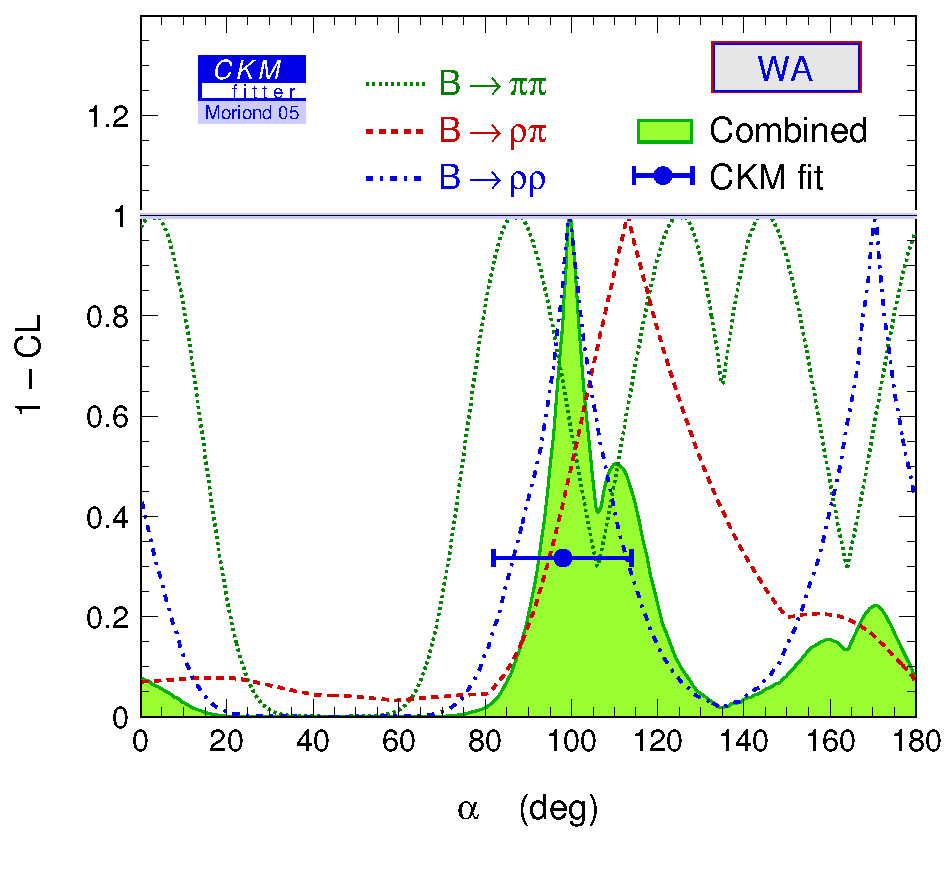
\includegraphics[width=\largefigwidth]{ckmfitter-alpha-combined}
%   \caption[CKM Fitter constraints on \alphaCKM.]%
%   {CKM Fitter constraints on \alphaCKM from combined \BToPiPi,
%     \BToRhoPi and \BToRhoRho decay analyses.}
%   \label{fig:CKMFitter}
% \end{figure}

\section{Supersymmetry}
\label{sec:susy}

% \begin{sidewaysfigure}
%   \begin{center}
%   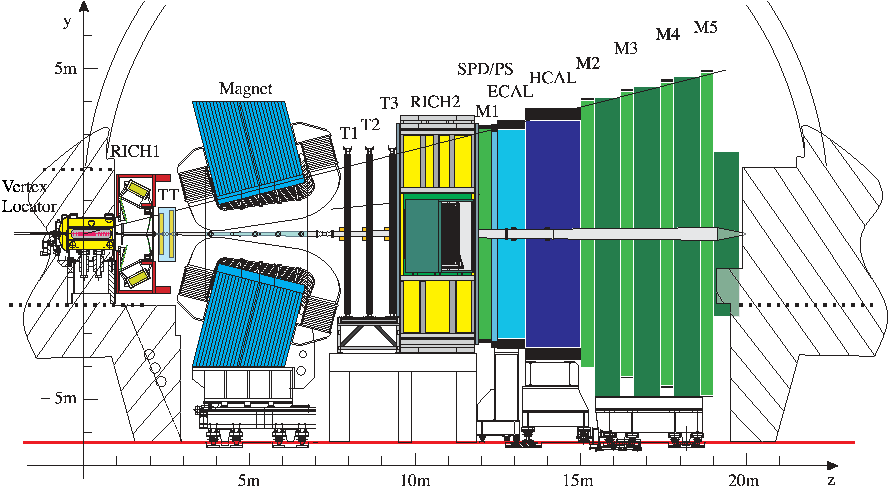
\includegraphics[width=0.8\textheight]{figs/example/lhcb-detector-cross-section}
%   \caption[Cross-section view of \LHCb, cut in the non-bending $y$--$z$ plane]%
%     {Cross-section view of \LHCb, cut in the non-bending $y$--$z$ plane.}
%   \label{fig:LHCbCrossSection}
%   \end{center}
% \end{sidewaysfigure}

\section{Signatures of supersymmetry at the LHC}

As the LHC is a hadron collider, the highest cross section SUSY
production processes occur via the strong force
\cite{Martin:1997ns}
\cite{SUSYxsections_NewAspectsof_pp_collisions}. These processes
result in the production of squarks and gluinos, the SUSY particles
with colour charge. In all favoured SUSY models, these relatively
heavy particles decay within the detector to a weakly interacting LSP,
usually a neutralino \cite{Farrar:1978xj}. In
collisions at the LHC this will appear as several hard jets with
unbalanced momentum (missing energy). 

%Decays etc.
